\documentclass{../paper}

\newcommand{\eq}[1]{Eq.~\eqref{#1}}
\newcommand{\eqs}[2]{Eqs.~\eqref{#1}--\eqref{#2}}
\newcommand{\fig}[1]{Fig.~\ref{#1}}

\newcommand{\todo}[1]{{\em [To-do: #1]}}

\begin{document}

\title{Quantum Optics \\ {\em Post-lab}}

\author{Iago B.~Mendes\,\orcidlink{0009-0007-9845-8448}}
\email{ibrazmen@oberlin.edu}
\affiliation{Department of Physics and Astronomy, Oberlin College, Oberlin, Ohio 44074, USA}

\date{\today}

\maketitle

General to-do's for the complete lab report:
\begin{itemize}
  \item Give a historical overview.
  \item Explain the quantum mechanical states better instead of simply mentioning the maximum entangled state in \eq{eq:entangled-state}.
  \item Mention the alignment process.
\end{itemize}

\section{Background}

In this experiment, we use non-linear optic properties of birefringent crystals to generate entangled photon pairs, which are then sent to a couple of detectors that are preceded by polarizers. If $\alpha$ and $\beta$ represent the angles from the detector polarizers to the vertical, it can be shown that the probability that both detections come out as ``vertical'' is given by
\begin{equation}\label{eq:Pvv}
  \begin{aligned}
    P_{VV}(\alpha, \beta)
    &= \sin^2\alpha \sin^2\beta \cos^2\theta_l \\
    &\quad + \cos^2\alpha \cos^2\beta \sin^2\theta_l \\
    &\quad + \frac{1}{4} \sin2\alpha \sin2\beta \sin2\theta_l \cos\phi_m
  \end{aligned}
\end{equation}
\cite{Dehlinger2002}, where $\theta_l$ represents the initial polarization of the laser beam and $\phi_m$ is an averaged accumulated phase shift.

In the maximally entangled state ($\theta_l = \pi/4$ and $\phi = 0$), \eq{eq:Pvv} reduces to
\begin{equation}\label{eq:Pvv-QM}
  P^\text{QM}_{VV}(\alpha, \beta) = \frac{1}{2} \cos^2(\beta - \alpha)
\end{equation}
\cite{Dehlinger2002}. However, if we consider a local realistic hidden variable theory (HVT), it can be shown that such maximally entangled state would lead to a probability of
\begin{equation}\label{eq:Pvv-HVT}
  P^\text{HVT}_{VV}(\alpha, \beta) = \frac{1}{2} - \frac{|\beta - \alpha|}{\pi}
\end{equation}
\cite{Dehlinger2002}.

In studying the feasibility of a HVT, John Bell derived an inequality that must be true for any HVT \cite{Bell1964}. In the context of \eq{eq:Pvv-HVT}, it was found in \cite{Clauser1969} that this inequality can be expressed as
\begin{equation}\label{eq:Bell-inequality}
  |S| \leq 2
\end{equation}
\cite{Dehlinger2002}, where
\begin{align}
  S &\equiv E(a,b) - E(a,b') + E(a',b) + E(a',b') \label{eq:S} \\
  E(\alpha,\beta) &\equiv P_{VV}(\alpha,\beta) + P_{VV}(\alpha_\perp,\beta_\perp) \label{eq:E-inP} \\
                  &\notag \qquad\qquad\quad - P_{VV}(\alpha,\beta_\perp) - P_{VV}(\alpha_\perp,\beta),
\end{align}
and the angles $a$, $b$, $a'$, and $b'$ are defined as in \fig{fig:angles}.

\begin{figure}
  \centering
  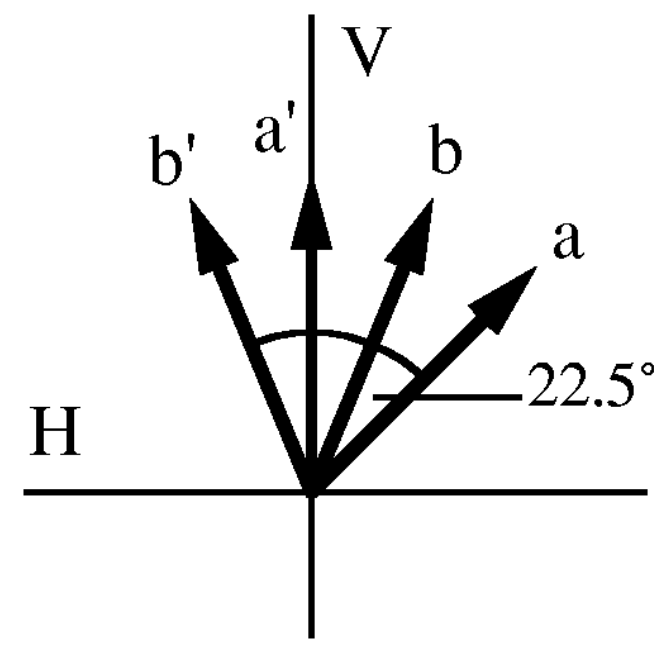
\includegraphics[width=0.6\columnwidth]{assets/angles.png}
  \caption{Schematic showing the angles used in \eq{eq:S}. Here, $a = -45\deg$, $b = -22.5\deg$, $a = 0\deg$, and $b' = 22.5\deg$. This figure is reproduced from \cite{Dehlinger2002}.}
  \label{fig:angles}
\end{figure}

This means that if a HVT exists, then \eq{eq:Bell-inequality} must be satisfied. However, if the quantum mechanical prediction from \eq{eq:Pvv-QM} is correct, then the value of $S$ will be greater than 2, violating \eq{eq:Bell-inequality}.

\section{Procedure}

It is important to note that Quantum Mechanics does not necessarily violate \eq{eq:Bell-inequality} in all cases. However, we have chosen the angles in \fig{fig:angles} such that the quantum mechanical prediction for $S$ is maximized (and greater than 2) in the maximally entangled state \cite{Dehlinger2002}, thus violating \eq{eq:Bell-inequality}.

Our experimental setup is shown in \fig{fig:setup}. A vertically polarized 407 nm laser beam is sent into a couple of wave plates. The half-wave plate (HWP) is used to rotate the polarization of the photons to be as close as possible to the desired angle $\theta_l = 45\deg$, while the quarter-wave plate (QWP) phase-shifts the photons so that we achieve the maximally entangled state. We will discuss how we have calibrated the angles of these wave plates later in the next section. If done correctly, the photons emerging from these wave plates will be in the maximally entangled state,
\begin{equation}\label{eq:entangled-state}
  \frac{1}{\sqrt{2}} (\ket{HH} + \ket{VV})
\end{equation}
\cite{LabManual}. If not done correctly, the photons will not be in the maximally entangled state, and the value of $S$ might not be help us in evaluating Bell's inequality.

\begin{figure}
  \centering
  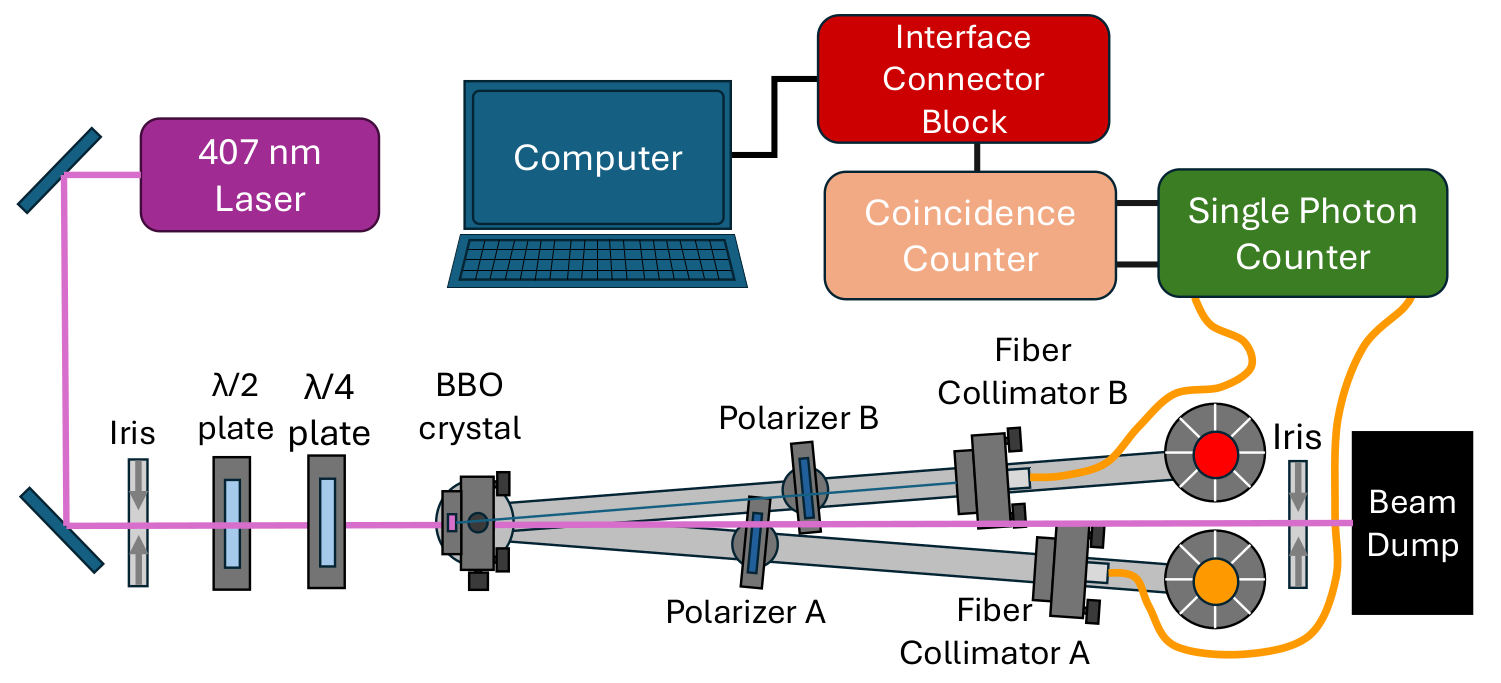
\includegraphics[width=1.0\columnwidth]{assets/setup.png}
  \caption{Experimental setup. This figure is reproduced from \cite{LabManual}.}
  \label{fig:setup}
\end{figure}

The entangled photons are then sent to a pair of beta barium borate (BBO) crystals, where they undergo spontaneous parametric down-conversion, producing two orthogonally polarized beams \cite{Dehlinger2002}. The two beams are then sent to polarizers at angles $\alpha$ and $\beta$ from the vertical. The photons are then detected by a couple of single-photon detectors. The detectors are connected to a coincidence counter, which records the number of times both detectors detect a photon at the same time in a coincidence window of $\tau = 25$ ns \cite{LabManual}.

The coincidence counter gives us $N(\alpha,\beta)$, the number of coincidences for a given configuration of the polarizers. We can re-write \eq{eq:E-inP} in terms of $N(\alpha,\beta)$ as
\begin{equation}\label{eq:E}
  \footnotesize
  \begin{aligned}
    E(\alpha,\beta) \equiv \frac{N(\alpha,\beta) + N(\alpha_\perp,\beta_\perp) - N(\alpha,\beta_\perp) - N(\alpha_\perp,\beta)}{N(\alpha,\beta) + N(\alpha_\perp,\beta_\perp) + N(\alpha,\beta_\perp) + N(\alpha_\perp,\beta)}
  \end{aligned}
\end{equation}
\cite{Dehlinger2002}. With this, we can calculate the value of $S$ using \eq{eq:S}.

It's important to note that we need to subtract background single-photon counts from our measurements. By blocking the beam path, we measured the background single-photon count rate in detector A $\dot N_A^\text{background} \approx 624$ Hz and in detector B $\dot N_B^\text{background} \approx 923$ Hz. After measuring the raw counts in both detectors ($N_A^\text{raw}$ and $N_B^\text{raw}$), we define
\begin{align}
  N_A &= N_A^\text{raw} - T \dot N_A^\text{background}, \\
  N_B &= N_B^\text{raw} - T \dot N_B^\text{background},
\end{align}
where $T$ is the duration of the measurement.

Additionally, we know from \cite{LabManual} that there is an expected number of accidental coincidences given by
\begin{equation}
  N^\text{ac} = N_A N_B \frac{\tau}{T}.
\end{equation}
After measuring the raw coincidences $N^\text{raw}$, we can then define the corrected coincidences as
\begin{equation}
  N = N^\text{raw} - N^\text{ac}.
\end{equation}

\section{Results}

\subsection{Calibration of wave plates}

To calibrate the HWP, we varied its angle from the vertical $\lambda_H$ and recorded $N(\alpha, \beta)$ in two configurations: $(\alpha,\beta) = (0\deg, 0\deg)$ and $(\alpha,\beta) = (90\deg, 90\deg)$. We then fitted the data to the expected shape of $\sin^2(\lambda_\text{HWP})$ using {\tt SciPy}'s {\tt curve\_fit} procedure \cite{SciPy}. The results are shown in the left panel of \fig{fig:wave-plates}. Seeking the state in \eq{eq:entangled-state}, we want to equalize $N(0\deg,0\deg)$ and $N(90\deg,90\deg)$, which is satisfied when $\lambda_H \sim 62\deg$.

We calibrated the QWP similarly. We varied its angle from the vertical $\lambda_Q$ and recorded $N(45\deg,45\deg)$, which we want to maximize. The resulting data and fit are shown in the right panel of \fig{fig:wave-plates}. From this, we see that the maximum of $N(45\deg,45\deg)$ is satisfied when $\lambda_Q \sim 140\deg$.

All of these measurements had a duration of $T = 30$ s.

\begin{figure*}
  \centering
  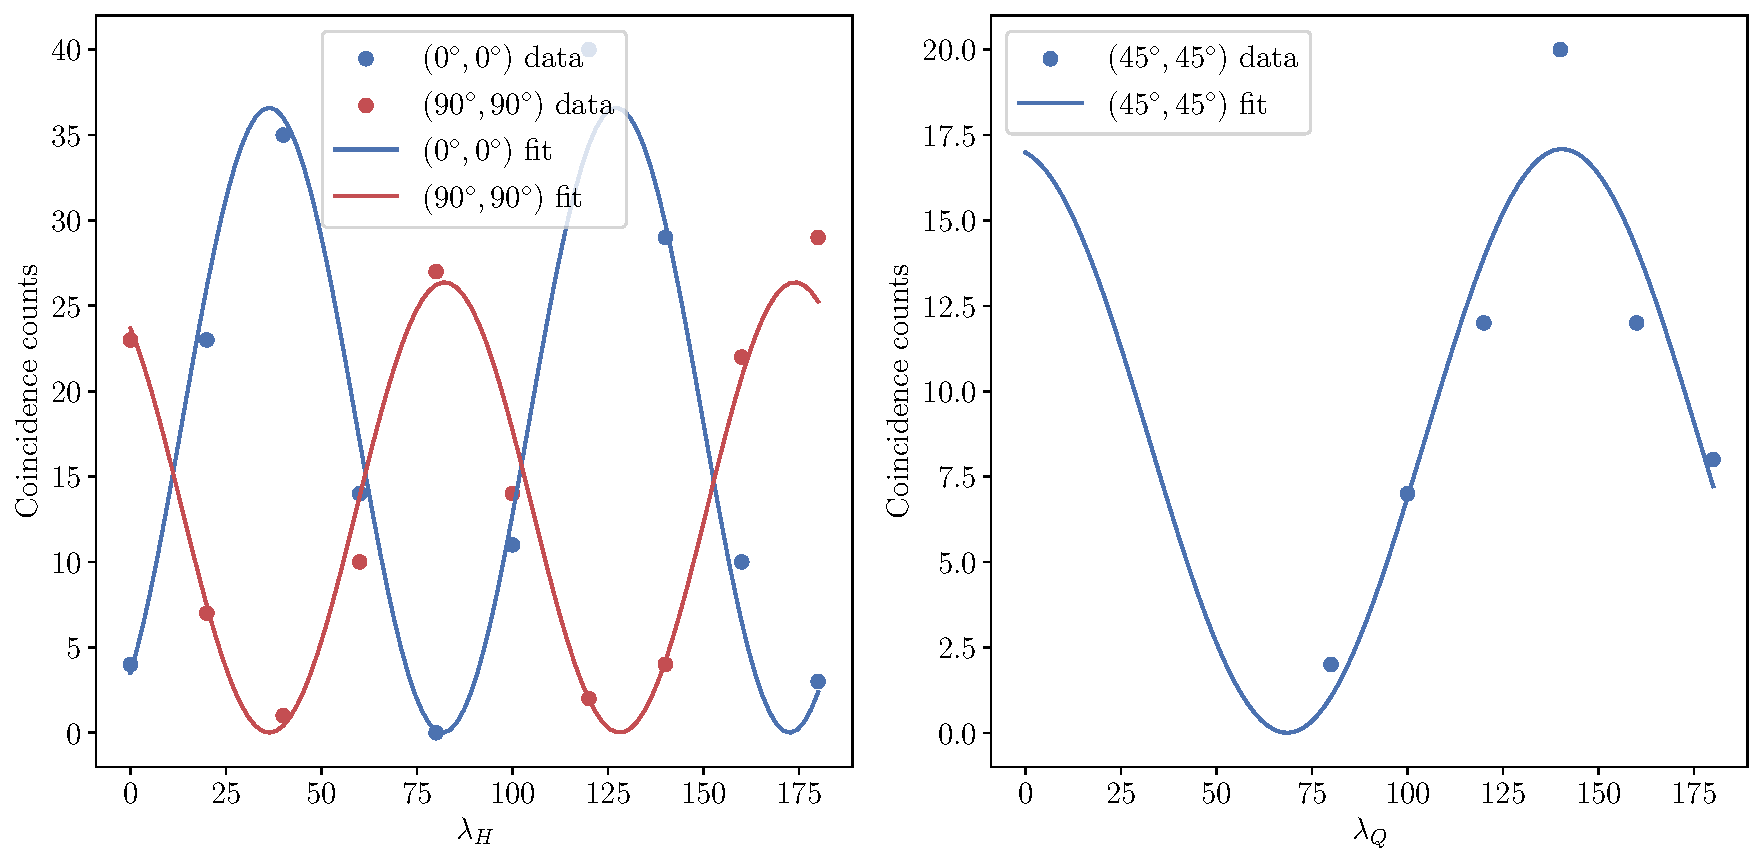
\includegraphics[width=0.6\textwidth]{analysis/wave-plates.pdf}
  \caption{Calibration of the HWP (left) and the QWP (right).}
  \label{fig:wave-plates}
\end{figure*}

\subsection{Analysis of state}

Our first set of measurements (shown in Table \ref{tab:5-measurements}) was taken with $T=60$ s in order to analyze our prepared state. Our second set of measurements (shown in Table \ref{tab:16-measurements}) was taken with $T=8$ minutes to be used in to evaluate $S$.

From \cite{LabManual}, we know that the expected number of coincidences can be modelled by
\begin{equation}\label{eq:N-model}
  \begin{aligned}
    N(\alpha,\beta)
    &= A (\sin^2\alpha \sin^2\beta \cos^2\theta_l \\
    &\qquad + \cos^2\alpha \cos^2\beta \sin^2\theta_l \\
    &\qquad + \frac{1}{4} \sin2\alpha \sin2\beta \sin2\theta_l \cos\phi_m) + C
  \end{aligned}
\end{equation}
and that $\theta_l$ can be estimated with
\begin{equation}\label{eq:theta_l}
  \tan^2\theta_l = \frac{N(90\deg,90\deg) - N(0\deg,90\deg)}{N(0\deg,0\deg) - N(0\deg,90\deg)}.
\end{equation}

Using the results from Table \ref{tab:5-measurements} in \eq{eq:theta_l}, we find
\begin{equation}\label{eq:theta_l-estimate1}
  \theta_l \approx 56\deg
\end{equation}
\todo{find uncertainty}. This clearly deviates from the desired $\theta_l = 45\deg$, which is likely due to improper calibration of the wave plates or misalignment of the other optical components.

In order to get a better estimate of the prepared state used in the data of actual interest, we can fit the measurements from Table \ref{tab:16-measurements} into a model like \eq{eq:N-model}. We performed such fit using {\tt SciPy}'s {\tt least\_squares} procedure \cite{SciPy}. The resulting fit is shown in the left plot of \fig{fig:state}. This fit gives us
\begin{align}
  A &\approx 196, \label{eq:A-estimate} \\
  \theta_l &\approx 25\deg, \label{eq:theta_l-estimate2} \\
  \phi_m &\approx 0.003\deg, \\
  C &\approx 19. \label{eq:C-estimate}
\end{align}
\todo{get uncertainties} Again, this is disappointly far from the desired $\theta_l = 45\deg$. The significant difference between \eq{eq:theta_l-estimate1} and \eq{eq:theta_l-estimate2} is concerning and should be investigated further in future experiments.

\begin{table*}
  \centering
  \begin{tabular}{ccccc}
    \hline
    \hline
    $\alpha$ & $\beta$   & $N_A^\text{raw}$ & $N_B^\text{raw}$ & $N^\text{raw}$ \\
    \hline
    $0\deg$  & $0\deg$   & $66195$          & $64087$	         & $10$           \\
    $90\deg$ & $90\deg$  & $76322$          & $97093$	         & $17$           \\
    $0\deg$  & $90\deg$  & $64369$          & $96829$	         & $4$            \\
    $45\deg$ & $45\deg$  & $74406$          & $86618$	         & $19$           \\
    $45\deg$ & $-45\deg$ & $73555$          & $76268$	         & $6$            \\
    \hline
  \end{tabular}
  \caption{Set of 5 measurements taken with $T = 30$ s.}
  \label{tab:5-measurements}
\end{table*}

\begin{table*}
  \centering
  \begin{tabular}{ccccc}
    \hline
    \hline
    $\alpha$  & $\beta$    & $N_A^\text{raw}$ & $N_B^\text{raw}$ & $N^\text{raw}$ \\
    \hline
    $-45\deg$ & $-22.5\deg$ & $548510$         & $565065$         & $76$          \\
    $-45\deg$ & $22.5\deg$  & $546175$         & $626254$         & $24$          \\
    $-45\deg$ & $67.5\deg$  & $546660$         & $807829$         & $63$          \\
    $-45\deg$ & $112.5\deg$ & $545895$         & $738278$         & $120$         \\
    $0\deg$   & $-22.5\deg$ & $522904$         & $522904$         & $48$          \\
    $0\deg$   & $22.5\deg$  & $520821$         & $625289$         & $37$          \\
    $0\deg$   & $67.5\deg$  & $519373$         & $808650$         & $27$          \\
    $0\deg$   & $112.5\deg$ & $522048$         & $744202$         & $19$          \\
    $45\deg$  & $-22.5\deg$ & $605777$         & $578021$         & $41$          \\
    $45\deg$  & $22.5\deg$  & $597014$         & $632914$         & $75$          \\
    $45\deg$  & $67.5\deg$  & $592238$         & $810973$         & $141$         \\
    $45\deg$  & $112.5\deg$ & $593777$         & $745974$         & $66$          \\
    $90\deg$  & $-22.5\deg$ & $623314$         & $568441$         & $39$          \\
    $90\deg$  & $22.5\deg$  & $617312$         & $620594$         & $45$          \\
    $90\deg$  & $67.5\deg$  & $619769$         & $817720$         & $175$         \\
    $90\deg$  & $112.5\deg$ & $621931$         & $746304$         & $139$         \\
    \hline
  \end{tabular}
  \caption{Set of 16 measurements taken with $T = 8$ minutes.}
  \label{tab:16-measurements}
\end{table*}

\begin{figure*}
  \centering
  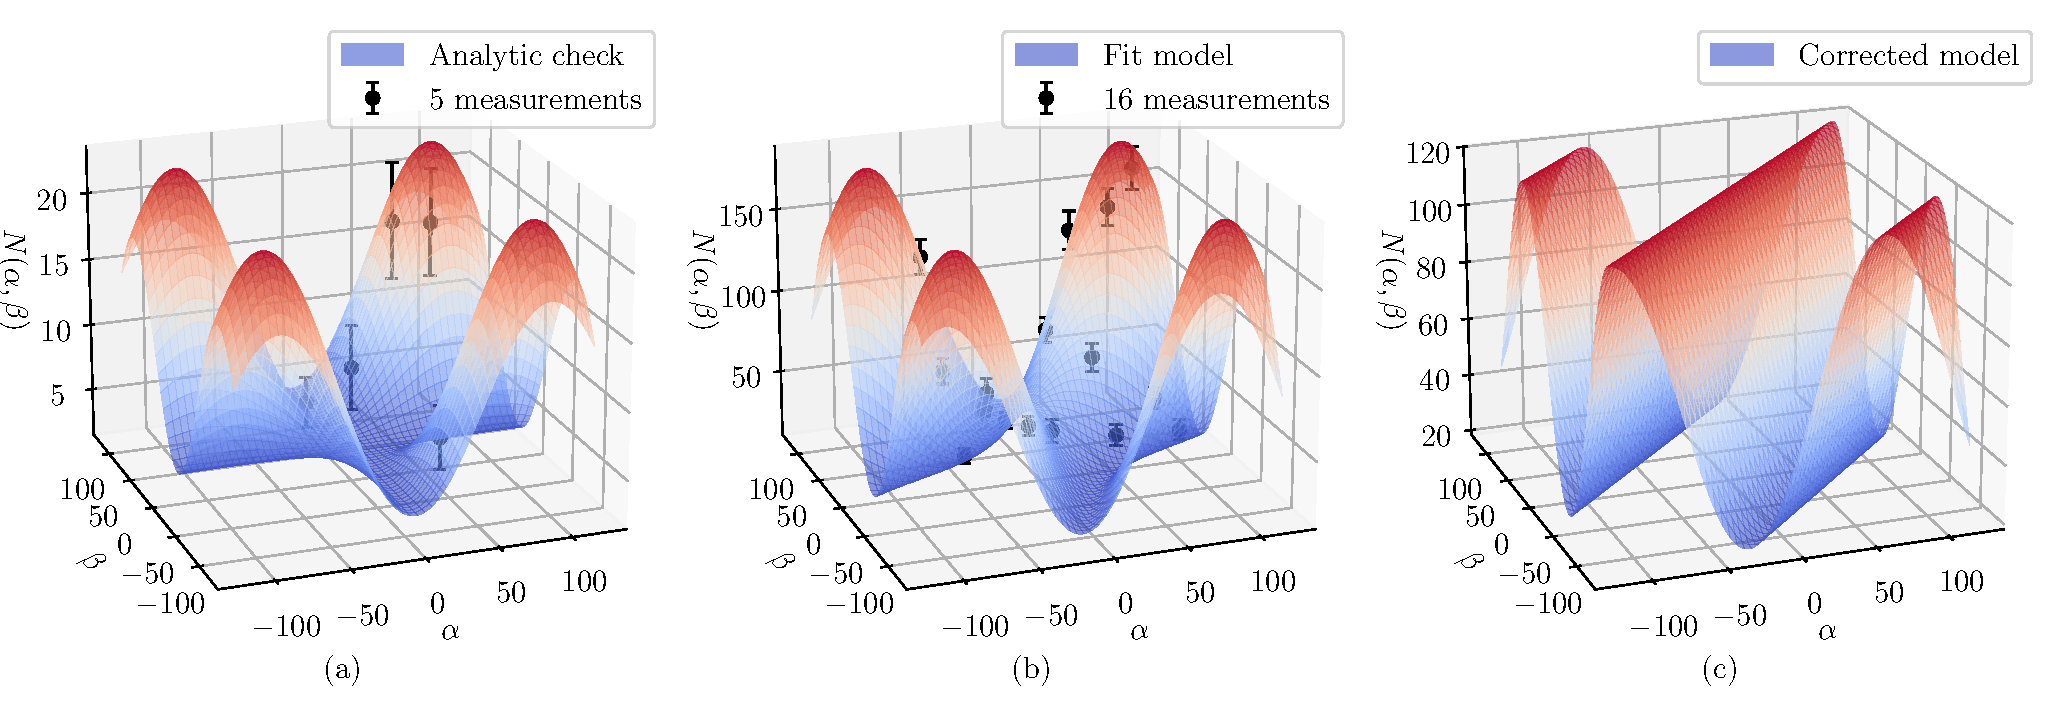
\includegraphics[width=0.8\textwidth]{analysis/state.pdf}
  \caption{Analysis of the state of the measurements in Table \ref{tab:16-measurements}.}
  \label{fig:state}
\end{figure*}

\subsection{Bell's inequality}

Using the measurements in Table \ref{tab:16-measurements}, we can calculate the value of $S$ using \eq{eq:S} and \eq{eq:E}. The resulting value is
\begin{equation}
  S \approx 1.8(1).
\end{equation}
Unfortunately, we do not get the expected violation of Bell's inequality, as this value is less than 2. This is likely due to the fact that we did not properly prepare the photons in the maximally entangled state, as discussed in the previous section.

That said, we can try to estimate what out $S$ value would be if we use our model from \eq{eq:N-model} with the parameters found in \eqs{eq:A-estimate}{eq:C-estimate}, except that we enforce that $\theta_l = 45\deg$. By doing this and re-calculating $S$ using \eq{eq:S} and \eq{eq:E}, we find
\begin{equation}
  S \approx 2.0(1).
\end{equation}
While this brings us closer to the expected violation of Bell's inequality, it is still not enough to conclude that we have violated \eq{eq:Bell-inequality} because of our uncertainty.

\begin{acknowledgements}
  This work was done in collaboration with Anya Molodtsova under the supervision of Professor Yuri Ijiri.
\end{acknowledgements}

\bibliography{refs}

\end{document}
